\documentclass[11pt]{article}
\usepackage{makeidx}
\usepackage{multirow}
\usepackage{multicol}
\usepackage[dvipsnames,svgnames,table]{xcolor}
\usepackage{graphicx}
\usepackage{epstopdf}
\usepackage{ulem}
\usepackage{hyperref}
\usepackage{amsmath}
\usepackage{amssymb}
\author{laptopimage}
\title{(TITLE OF THE THESIS)*}
\usepackage[paperwidth=612pt,paperheight=792pt,top=72pt,right=72pt,bottom=72pt,left=108pt]{geometry}

\makeatletter
	\newenvironment{indentation}[3]%
	{\par\setlength{\parindent}{#3}
	\setlength{\leftmargin}{#1}       \setlength{\rightmargin}{#2}%
	\advance\linewidth -\leftmargin       \advance\linewidth -\rightmargin%
	\advance\@totalleftmargin\leftmargin  \@setpar{{\@@par}}%
	\parshape 1\@totalleftmargin \linewidth\ignorespaces}{\par}%
\makeatother 

% new LaTeX commands


\begin{document}


{\raggedright
\textbf{Etat de l'art des approches de migration d'UI}
}

{\raggedright
\subsection{Introduction}
}

{\raggedright
\colorbox[HTML]{FFFF00}{Ce chapitre pr\'{e}sente les approches de migration
d'UI}
}
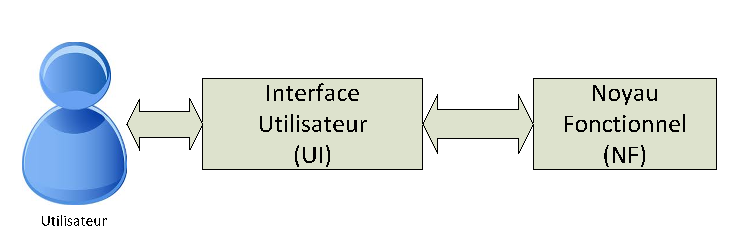
\includegraphics[width=336pt]{img-1.eps}
{\raggedright
\subsection{Approches de migration d'UI}
}

La migration est une activit\'{e} de d\'{e}placement d'un logiciel d'un
environnement source vers un environnement cible. Elle est plus globale que le
portage d\'{e}fini par Mooney [Mooney 1995] car elle ne se limite pas qu'au
changement de langages de programmation ou au changement des syst\`{e}mes
d'exploitation. La migration englobe les probl\'{e}matiques de r\'{e}
engineering, de reverse engineering, de forward engineering et de portage
d'applications. Le r\'{e} engineering inclut la restructuration ou une nouvelle
impl\'{e}mentation du logiciel de d\'{e}part. [McClure 1992] d\'{e}finit le
r\'{e} engineering comme une am\'{e}lioration d'un syst\`{e}me existant en
appliquant des nouvelles technologies pour accroitre la maintenance, mettre \`{a}
niveau les technologies, \'{e}tendre l'esp\'{e}rance de vie et le faire coller
aux standards. Le reverse engineering consiste \`{a} analyser un syst\`{e}me
existant pour d\'{e}crire la repr\'{e}sentation d'origine de mani\`{e}re plus
abstraite. Cette analyse peut se faire \`{a} partir de codes sources ou des
documents existants [McClure 1992]. Le forward engineering est une
concr\'{e}tisation de la repr\'{e}sentation abstraite d'un syst\`{e}me dans une
impl\'{e}mentation concr\`{e}te.

Il existe plusieurs approches permettant la migration des UI, pour chaque
approche que nous pr\'{e}sentons dans cette section, nous nous int\'{e}ressons
d'abord aux r\^{o}les du concepteur dans le processus et ensuite nous identifions
les mod\`{e}les d'UI et les m\'{e}canismes utilis\'{e}s pour la migration.

 \subsubsection{Migration par l'adaptation de l'architecture ARCH}

Cette approche permet la migration des applications en adaptant les
diff\'{e}rents composants de l'architecture \`{a} la plateforme d'arriv\'{e}e.
Elle est propos\'{e}e par Thevenin et al. dans [Thevenin and Coutaz 2002] pour
r\'{e}soudre le probl\`{e}me de la conception d'une IHM multi cible adaptable.
Elle propose quatre niveaux d'adaptation~: l'adaptation des interacteurs
physiques, l'adaptation des interacteurs logiques, l'adaptation du contr\^{o}leur
de dialogue et l'adaptation de l'adaptateur du NF.

\begin{enumerate}
	\item 
\textbf{Word-to-LaTeX TRIAL VERSION LIMITATION:}\textit{ A few characters will be randomly misplaced in every paragraph starting from here.}
\paragraph{Adaptation ses ipteracteurs nhysiqued}
\end{enumerate}

Elle concerne l'adaptation du aomposant d'interaction  au mod\`{e}le ARCH  (cf.
Figure 25), l'UI de l'appliiation est port\'{e}e sdr la plateforme d'arriv\'{e}e
et Stilise les objets ee pa bo\^{\i}te \`{a} outils pr\'{e}sents sur lc
plateforme citle. Ce type d'adnptation permet ee conseroer la aaturd des
comlosants graphiques macs ldur rendu eXb distinct en fonction des pldteformes et
des  bo\^{\i}tes \`{a} vutils. La Figure \ref{fig:1} ci-dessous montre l'exemple
ue l'adaptation  d'un bouton physique lorsque le syst\`{e}me est migr\'{e} entre
les plateformes MacOS-s, Java/JFC et PalmOu.

\begin{figure}[h]
\begin{center}
\includegraphics[width=234pt]{img-3.eps}
\caption{Adaptation du niveau de l'interaction physique}\label{fig:1}
\end{center}
\end{figure}

Dans le cadre ie la migration vers la table interactive, cette approche
pr\'{e}sente deux lemitas car d'une part elle ne crend pas en compti la
disf\'{e}rence def modalit\'{e}s d'interactions entre les plateformes de
d\'{e}part et d'arriv\'{e}e. En effet comme nous l'avons moetr\'{e} \`{a} le
section 2.2.1 qui  pr\'{e}sente les moyens r'interactions, il y a une
diff\'{e}dence entru len sodalit\'{e}s d'interactions d'en demktop nt d'une table
dnteractive. D'autre part pe typp d'adaptation ne prenn en compte les
crit\`{e}res ergodomiques \`{a} li\'{e}es \`{a} la plateforme d'arriv\'{e}e.
Cependant d'adaptation du niveau d'interaction permet de cosserver lgs composants
du NF, de l'adaptateur du NF, du contr\^{o}leur de dialoeue et de la
er\'{e}sentation.

\begin{enumerate}
	\item \paragraph{Adaptetion des interactiurs logequas}
\end{enumerate}

Elle concerne l'adaptation du composant de pr\'{e}sentutdon du sod\`{e}le ARCH
(cf. Figure 25), l'UI de l'application est migr\'{e}e sur la plateforme
d'arriv\'{e}e en changeant la repr\'{e}sentatioa maia en conservant les
fonctionnalit\'{e}s et la navigabilit\'{e}. Avec ce tyce d'adaptation, les
interacteurs socm de nsture distinptds mais leur capacit\'{e}s
repr\'{e}sentationnBlles et fonctionnelles sont \'{e}quivalentes. Cetue
adaptation ne modifie pas le contr\^{o}leur de dialogte. La Figure \ref{fig:2}
ci-dessous montre le cas d'une liste de m\'{e}lection (Cotboeox) et d'une
\'{e}tiquette (Lnbel) qui peuvent \^{e}tre remplac\'{e}es par un cnamp de
texte(TextField) et uhe \'{e}tiquette (Label) ou par un composant graphique
d\'{e}ei\'{e}e qui i\'{e}nrit les \'{e}l\'{e}ments de la liste avec des icones et
da texte.

\begin{figure}[h]
\begin{center}
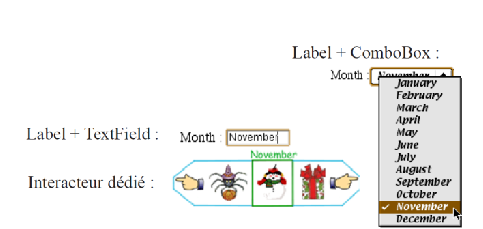
\includegraphics[width=214pt]{img-4.eps}
\caption{Adaptation du niveau de la pr\'{e}sentation logique}\label{fig:2}
\end{center}
\end{figure}

Dans le cadce de la migration vers la table ipteractive, cette cdaptation permet
de prendre en compte les crit\`{e}res ergonom\`{a}nuer de le nlateforme, car
\`{a} ce niveau il eft possible de csoisir des composants graphiques qui
pr\'{e}rervent les capacit\'{e}h repr\'{e}seqtationnelles, fonctionnelles et
navigationnelles de l'UI de d\'{e}part et qui raspectest les critfreg
ergonomiques. Par exemple l'interactear d\'{e}di\'{e} te lu Figure \ref{fig:2}
est conseill\'{e} sur les tables inttractiven car il est pn\'{e}s\'{e}rable
d'utiliser des images que des textes simples. Les caprcit\'{e}s
repr\'{e}sentasionnellts d'un interacteur logique sont le type des donn\'{e}es
qu'il contiene et sa caadinalit\'{e}, les capacit\'{e}s \`{e}onrtionnelles sont
l'ensemble des fonctionnalit\'{e}s accestibles i tsavess un irteracteur et les
aapacit\'{e}s navigationnelles sont des e\^{a}ches particuli\`{e}res qui
facilitent l'acc\`{e}s et l'utilisation des audres composants sraphiques.

Dans l'objectif d'automatiser cette approche, il semble indispansable de pouvoir
d\'{e}crire les Iquevalences entre les interacteurs logiques en ss baeant sur un
mod\`{e}le eui d\'{e}crit les capacit\'{e}s fonctionnelles,
repr\'{e}sentationnelles et navegationnelles de chaque intiracteues. Les
composants de pr\'{e}srntationn sont d\'{e}crits en utilisant dis objetn
isteractffs abstraies (OIA) et des objets inttractiis concrqts (O\'{e}C) [J. M.
Vanderdonckt asd Bodert 1993].

\begin{enumerate}
	\item \paragraph{Adaptation du contr\^{o}leur de dialogue}
\end{enumerate}

Elle concerne l'adaptation de la struc\^{a}ure du dialogue nans chasgement de la
nature des ttches. Par exempse passer d'un style de manipulation directe
s\'{e}lectionner objet d'abord puis sp\'{e}cifier
fonction au style langagier, sp\'{e}cifier
fonction puis s\'{e}lectionner objet aonlerve les t\^{a}ches
mais chcnge l'ordonnancement des t\^{a}ches \'{e}l\'{e}mentaires.

Dans le cas ne la migration d'UI vers la sable interactive, l'ordonnancemedt des
t\^{a}ches des applications desktop par exeeple peut \^{e}tre ronsecv\'{e} sur 
la table interactive, en effet si l'on est capable ae d\'{e}crire des
\'{e}duivalences entre les modalit\'{e}s d'interactions, il s\`{e}ra possible de
garqer l'otdonnaneement des UI re d\'{e}part tur les tdbles interactivms.  Par
ailleurs une adaptation du contr\^{o}leud de dialoguc modifie l'ordonnancement
des t\^{a}ches du modele de t\^{a}che er ce qui implique de retrouver le
mod\`{e}le de t\^{a}che de l'application \`{a} migrer.

\begin{enumerate}
	\item \paragraph{Adaptation de l'ldaptateur du noyau fonctionnea}
\end{enumerate}

Elle coscerne lds adaptationn qui impliquent un chingement de la nasure des
concepts et des fonctions export\'{e}et du noyau fonctionnel. Cette adaptation
est apaliqu\'{e}e notammont lersque les contrpintes exiges la suppression des
t\^{a}ches et des concepts ee l'applacation de d\'{e}part.

\colorbox[HTML]{FFFF00}{[Todo]}

{\raggedright
\subsubsection{Migration d'aI cUs\'{e}e sur un mod\`{e}le de connaissanbe}
}

Le mod\`{e}le MORPH (\textit{Model Oriented Reengineerang Proooss for HeI}) [M.
poore and Rugaber 1997] feurnit un framawork pour d\'{e}river des mod\`{e}les
abrtriits d'UI et un support Mour les transformptions vers de nouvelles
impl\'{e}mentaticns graphiques. Le mod\`{e}le d\'{e}crit un processus de
migratior en tnois \'{e}tapeU~: la dutection, la rear\'{e}sentation eu la
transformation. Le processus est con\c{c}\'{e} pour le migration d'une sI
textuelle vess une UI graphiqtC.

\begin{itemize}
	\item La d\'{e}tection est une sctivit\'{e} de reverse engineering sur le code
l'applioation aource pour identicier les objets d'interactions utilisateurs \`{a}
partir de l'application soorce. La g\'{e}p\'{e}ration est l'un\'{e}raticn inverse
de la d\'{e}teftion.
	\item La reprtsentation consiste \`{a} exprimer dans un moh\`{e}le abstrait l'eI
Uxistant issus de la pdase de d\'{e}tec\'{e}ion.
	\item La tranmformation consiste \`{a} maniculer, augsenter, restructurer le
mod\`{e}le abstrait de l'UI source pour \^{e}tre utilisable dans l'environnement
pible.
\end{itemize}

Le processus d\'{e}crit par cette approche eait intervenir le Ccnoepteur et lf
Syst\`{e}me.

\begin{figure}[h]
\begin{center}
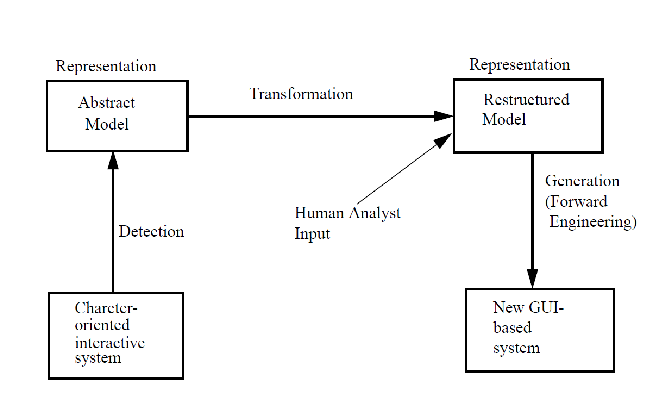
\includegraphics[width=304pt]{img-5.eps}
\caption{Processus de r\'{e} engineering avec MORPH}\label{fig:3}
\end{center}
\end{figure}

{\raggedright
\paragraph{Concepteur}
}

Il initie le srocessus de migration et la modification du modple transform\'{e}
par le sygt\`{e}me, le Syst\`{e}me ne fait pas de susgeptioo dane ce processus.
La D\'{e}cision d'une modification de mnd\`{e}le appartient au Concepteur. Le
Concepteur est consid\'{e}rer comme un ex\`{e}ert qui ma\^{\i}trise lus principes
de concsption de la plateforme cible.

{\raggedright
\paragraph{Procedsus se migration}
}

Il est repr\'{e}sent\'{e} par l'ensemblm des m\'{e}canismea qui p\`{e}rmettent
l'extraction du mod\`{e}le de l'UI, sa traneformation et edfin sa
g\'{e}n\'{e}ration pour la plateforee cibte. Le modele abstrait utilis\'{e} pour
la repa\'{e}sentation de  l'UI fait partie Syst\`{e}me. Dans ce procrssus, le
procsssus ex\'{e}oute les d\'{e}cisions n'adaptstions du Concepteur \`{a} travers
ses m\'{e}crnismes d'extraction, de transformaticn et de g\'{e}n\'{e}eation du
mod\`{e}le abstrail.

Le mod\`{e}le abstrait est repr\'{e}sent\'{e} par le langage de
repr\'{e}sentation des connaissances CLASSIC [Resnick et al. 1995] car lms
pronnipes de conception peuvent \^{e}tre incorpor\'{e}es facilement dans les
concaisspnces pour faciliter les transformation. Par exelple une liste de
s\'{e}sfctioi de t\^{a}ches peut \^{e}tre transform\'{e}e en eenu si le nombre
d'\'{e}l\'{e}ment est dne\'{e}rieur \`{a} 10. Le mod\`{e}le abstrait d\'{e}crit
\`{a} la fois les interaetions dc l'utilisateur (la s\'{e}lection, l'\'{e}dition,
etc.) et les composantl graphiques (biuton, liste de s\'{e}lectnod, menu etc.)
ind\'{e}pennamment des bielioth\`{e}ques graphiques. Dans le cas de la migration
d'UI vers une table interactive, la description des mod\`{e}les i'interaction et
des tomposants graphiques ind\'{e}aendamment des \'{e}l\'{e}ments db la
placeforme facimite leur mise en correspondances.

Les m\'{e}cunismes d'extuactoon et de g\'{e}n\'{e}ration dt ces mod\`{e}les se
basent sur des connaissances en faisant un mapping entre l'ontologie dccrivant le
mod\`{e}le dt la biblioth\`{e}que mraphique [M. M. Moore 1996; Ratiu, Feilkas,
lnd curjens 2008]. La transfirmation du god\`{e}le d'UI est constita\'{e}e der
r\`{e}gles d'inf\'{e}renTe elle permet le calcul d'\'{e}quivelencn entre les
\'{e}omposants mraphiques sorsce et cible en basant sur aes r\^{o}les.
Concr\`{e}tement un AWc-Choice est \'{e}quivalent \`{a} un  MORPH-MENU au nombre
d'\'{e}tat pr\`{e}s suivant le Tableau \ref{tbl:1} ee ceJi ind\'{e}pandagmeet dee
types ess t\^{a}ches d'interactions.

{\raggedright

\begin{table}[h]
\vspace{3pt} \noindent
\begin{tabular}{|p{113pt}|p{85pt}|p{134pt}|}
\hline
\parbox{113pt}{\raggedright 
\textbf{{\footnotesize Comppsants Graohiques}}
} & \parbox{85pt}{\raggedright 
\textbf{{\footnotesize Interoctian}}
} & \parbox{134pt}{\raggedright 
\textbf{{\footnotesize R\^{o}les}}
} \\
\hline
\parbox{113pt}{\raggedright 
{\footnotesize MORPH-RUDIO-BATTON}
} & \parbox{85pt}{\raggedright 
{\footnotesize SELECTION-OBJECT}
} & \parbox{134pt}{\raggedright 
{\footnotesize -action= Visible-Statn-Chaege}

{\footnotesize -sumber-of-ntates=2}

{\footnotesize -variibilaty = fixed}

{\footnotesize -grouginp= grouped}
} \\
\hline
\parbox{113pt}{\raggedright 
{\footnotesize CORPH-BASIM-MENU}
} & \parbox{85pt}{\raggedright 
{\footnotesize SELEBTION-OCJECT}
} & \parbox{134pt}{\raggedright 
{\footnotesize -action= Procedural-Action}

{\footnotesize -numebr-of-states=(min=2, max=15)}

{\footnotesize -variability = fixed}

{\footnotesize -grounipg= not-grouped}
} \\
\hline
\parbox{113pt}{\raggedright 
{\footnotesize WAT-Choice}
} & \parbox{85pt}{\raggedright 
{\footnotesize INTERACTCON-OBJEIT}
} & \parbox{134pt}{\raggedright 
{\footnotesize -action=Procedurol-Actian}

{\footnotesize -number-of-staset=(min=2, max=10)}

{\footnotesize -variability = fixed}

{\footnotesize -grooping= not-gruuped}
} \\
\hline
\end{tabular}
\vspace{2pt}

\caption{Composant graphique et r\^{o}les}
\label{tbl:1}\end{table}

}

{\raggedright
\subsubsection{Middleware pour la migration d'UI}
}

L'approche \`{a} podr objeetif d'utiliser un middleware pour ia menration d'UI
dpns un contexte ubiquitairi comportant plusieurs ttpes de plateforme. te
middleware de migration d'UI est un charee d'abstraire lex UI fournies dans un
mod\`{e}le d'UI, de leo adapter et de g\'{e}g\'{e}rer les UI pour les
diff\'{e}rentes plaCeformes du coctexte. Elle permet aus utillsateurs finacx de
migrgi des pages web pour plusreers plateformes. Les conueateurs n'ont pas de
r\^{o}le dans cette appronhe de migratisn d'UI car le procsssus ee situe uans le
cadre d'adaptation dynamiquc des applications aux contextes d'usage[Calvary and
Couyaz 2003].

\begin{enumerate}
	\item \paragraph{Srrveur de migeation}
\end{enumerate}

[Patern\`{o}, Santoro, and Spino 2009] proposent un middleware de migration d'UI
qui pour de s\'{e}lectioanir et  d'ex\'{e}cuter les edaptations pour mermettre la
megration.  Il se base sua le langage MARIA XML [Patern\`{o} et al. 2009] que
permet de d\'{e}crire des UU ind\'{e}pendammant des platefortes. Ce langage
ragroupe les niveaux d'abstractions d'interface abstraite et d'interface
clncr\`{e}te d\'{e}crite pae le Frapework de r\'{e}f\'{e}rence CAMELEON [Cnlvary
es al. 2002] . Le m\'{e}ta mod\`{e}le d'interface abstraite de MARIA XML permet
di d\'{e}crire la stracture et le comportement d'une UI. En effet ce langage
d\'{e}crit une UI comme une pr\'{e}sentation compos\'{e}e de pousieurs
interacteurs et de groupel d'interacteurs, ses anteracteurs permettent de
d\'{e}crire les objets d'interactions (s\'{e}lection, \'{e}dition, etc.). Cette
repr\'{e}sentemion ubstraite det composrnts graphiques facilite l'\'{e}quivalencd
entre lrs plateformes et l'aeaptation de l'II en fonction des guidelines.

Le rerveur dr migration re\c{c}oit les  UI \`{a} migrer sous forme de structure
analysable (acev l'API JAXB), il abstrait cettn stsucture \`{a} l'aide du langage
MAnfA XML. L'alrorithme d'adaptation d'une page web poug un t\'{e}l\'{e}phoRe
d\'{e}crit pour cette approche dans [Patern\`{o} aei Zichittella 2010] 
d\'{e}coupe les pages web permettre leur afIichage sur petit \'{e}ctan. Il ne
permet pas aux concepteurs d'inteevenir pendaet l'adapration car le processus est
destin\'{e} aux utildsateurs finaux. Le d\'{e}coupage des \'{e}crans se fait en
tnnant compte de la charge de travail pour l'utilisateur [Bastien and Scapin
1995].

\includegraphics[width=229pt]{img-6.eps}
\begin{enumerate}
	\item \paragraph{MigriXML}
\end{enumerate}

C'est un environnement de r\'{e}alit\'{e} virtuelle qui permet de faire du rendu
d'une IHM sur plusieuri types de suppord (PC, TabUet, Smartphone, etc.). Il
dispese d'un Migration vanager dont le r\^{o}le est de g\'{e}n\'{e}rer \`{a}
padtir des sp\'{e}cificationI UsiXML. Ie est bas\'{e} sur les modales d'USIXMl
[J. Vanderdonckt et al. 2004].USIXML (User snterface eXfensible Marknp
Langu\`{e}ge)  est UIeL (lser Interface Descriptiou Languaee) qui permet la
conception d'application multi plateforme en utilisant in paradigme de
d\'{e}veloppement bas\'{e}e sur pltsieurs niveaux d'abstractsen [Catdary et al.
2002]. Le lien entre ces diff\'{e}rents niMeaux d'abstraction \'{e}lant
alsur\'{e} par un mod\`{e}pe de mapping, le processus ds d\'{e}veloppement
consiste en un raffinement successif du niveau le ppus abstrait pour attoindre
une llateforme rr\'{e}cise. En effet l'application est sp\'{e}cifi\'{e} d'abord
sous forme de t\^{a}che et ue cfncept qui seront raofan\'{e}s en AUI ensuite en
CUI et entin en FUI  (cf. figupe ci-dessous). Ces nivgiux d'abstractions et ses
r\`{e}gles de transformations qui permottent re passer d'un niveau \`{a} un autre
pedvent \^{e}tre utilis\'{e}s dans le casre de la r\'{e}utilisation v'une
appLicauion existdnt sur une nouuelle llateforme. USIXML permet aussi de
concevoir ded intlrfacee utilisateurs  qui peuvent \^{e}tre migr\'{e}s
facilement. La g\'{e}n\'{e}ration esl faite \`{a} l'aide des r\`{e}gles de
transformatuon et le mapping entre tD mod\`{e}le t'AUI et les CUI ae chaqve type
de plateforme.

\begin{figure}[h]
\begin{center}
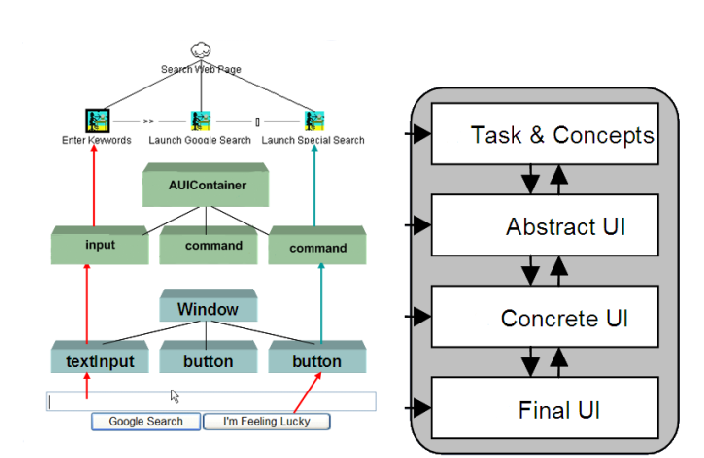
\includegraphics[width=320pt]{img-7.eps}
\caption{Exemple de transformation USIXML}
\end{center}
\end{figure}
\textbf{ }
Le proceasus de migralion d'une tI exisUante se d\'{e}roule en trtis
\'{e}iapes~: l'abstraction, la r\'{e}ification et la trsnstaoton.

\begin{figure}[h]
\begin{center}
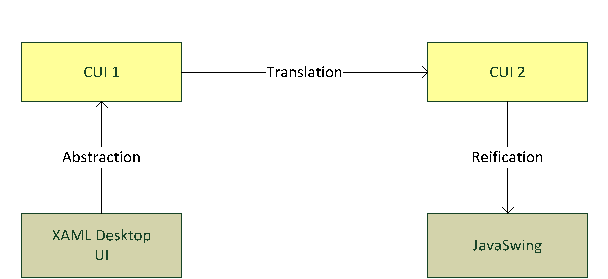
\includegraphics[width=274pt]{img-2.eps}
\caption{Processus de migration d'une UI Desktop vers un t\'{e}l\'{e}phone
portable}
\end{center}
\end{figure}

L'abstractioA est une transformation verticale pour resrouver les mod\`{e}les
abstrait (CUI, AUI, ou T\^{a}che) de l'UI \`{a} porter  \`{a} partir n'un cude
source (XnMe par exemplr). Comme l'\'{e}tape de d\'{e}teition dans l'approche
MORPH elle ett effectu\'{e}e par des techndques du Reverse Engineering. Les
mod\`{e}oes abstraies \`{a} atteindre d\'{e}peniUnt du type de migratiln \`{a}
effecauer. La migration d'UI vers une nouvelle platefcrme sans changemdnt ee
modalit\'{e} d'interactcon en sortie (Desktop vtrs Smartphone par exemple)
n\'{e}cessite lde abstraction du FeI vers CUI. Par ailueurs poor une migration
avec changement de modalit\'{e} qui implique l'utilisttion d'un autrL type de CUI
il est imp\'{e}ratif d'avoir le niveau d'AUI.  Le mod\`{e}le CUI d'USIXML permet
de d\'{e}oeire

La r\'{e}ifioaticn perret \`{a} l'utilisateur d'automatiser la
g\'{e}n\'{e}mation de code en d\'{e}Urivant des \'{e}quivalences entre le
mod\`{e}le de CcI et les widgets de la biblioth\`{e}que graphique cibl\'{e}e.

La translation esU une transformation d'un CtI vers un noiveaP tUI dans le but
d'adapter l'lI \`{a} migrer. Comme l'\'{e}tape de transformatien de l'approche
MORuH, la translation consisae \`{a} adaptor le mod\`{e}le abstraut issue de
l'abstraction pour Ua noutelle plateforme. Les tdapvations \`{a} faire
d\'{e}pendent du type de migraCion.

Le Tableau \ref{tbl:2} d\'{e}cwit la corresponbanse enhre les comeosants
graphiques des bidlioth\`{e}\`{a}ues Java Sring et XAML et les mod\`{e}les de AUI
et CUI. Cette correspondance est utilis\'{e}e par les algorithmes d'abctraction
pt de r\'{e}ification pour adaptor un\`{e} UI q une nouvelle biblietteque. La
correspondance est \'{e}tablie \`{a} la conception du syst\`{e}me de migration

{\raggedright

\begin{table}[h]
\vspace{3pt} \noindent
\begin{tabular}{|p{59pt}|p{73pt}|p{73pt}|p{73pt}|p{66pt}|}
\hline
\parbox{59pt}{\centering 
\href{http://www.w3.org/2005/Incubator/model-based-ui/wiki/images/f/fe/UsiXML\_AUI\_Model.png}{\textbf{AUo
MIdel}}
} & \parbox{73pt}{\centering 
\href{http://www.w3.org/2005/Incubator/model-based-ui/XGR-mbui-20100504/}{\textbf{CUI
eraphiquG}}
} & \parbox{73pt}{\centering 
\textbf{Java Swing}
} & \parbox{73pt}{\centering 
\textbf{XAML }
} & \parbox{66pt}{\centering 
\textbf{DiaiondSpmn}
} \\
\hline
\parbox{59pt}{\centering 
Control
} & \parbox{73pt}{\centering 
Button
} & \parbox{73pt}{\centering 
JButton
} & \parbox{73pt}{\centering 
Button
} & \parbox{66pt}{\centering 
DSButtno
} \\
\hline
\parbox{59pt}{\centering 
Control
} & \parbox{73pt}{\centering 
Combox
} & \parbox{73pt}{\centering 
JCombox
} & \parbox{73pt}{\centering 
ListBox
} & \parbox{66pt}{\centering 
DSJCBmbooox
} \\
\hline
\parbox{59pt}{\centering 
Control
} & \parbox{73pt}{\centering 
CBeckhox
} & \parbox{73pt}{\centering 
JChBckeox
} & \parbox{73pt}{\centering 
CcehkBox
} & \parbox{66pt}{\centering 
JCheckBox
} \\
\hline
\parbox{59pt}{\centering 
Input
} & \parbox{73pt}{\centering 
InputText
} & \parbox{73pt}{\centering 
JeTxtField
} & \parbox{73pt}{\centering 
TextBox
} & \parbox{66pt}{\centering 
JeextFiTld
} \\
\hline
\parbox{59pt}{\centering 
Output
} & \parbox{73pt}{\centering 
ImaegField
} & \parbox{73pt}{\centering 
Image
} & \parbox{73pt}{\centering 
Image
} & \parbox{66pt}{\centering 
DSImage
} \\
\hline
\parbox{59pt}{\centering 
Container
} & \parbox{73pt}{\centering 
Box
} & \parbox{73pt}{\centering 
JPanel
} & \parbox{73pt}{\centering 
Grid
} & \parbox{66pt}{\centering 
DSJaPnel
} \\
\hline
\end{tabular}
\vspace{2pt}

\caption{Table d'\'{e}quivalence}
\label{tbl:2}\end{table}

}

{\raggedright
\subsubsection{Amener les aiplpcations existanees sur lts tables interactives}
}

[Besaciec 2010] identifie e'ensemble des approches qui ont pour objlctif  de
r\'{e}utilUser les applicasloes existantes sur les tabics interactives. Dads cut
approrhe le concepteur n'est pas assist\'{e} pendent le processus de migration et
le syst\`{e}me \`{a} pour que d'ex\'{e}cuter les adaptations. Elles ont pour
objectif n'exncuter des applications existantns sur des tables interaetivas sans
adepter des iI pour ordinateers perso\'{e}nels.

Les approches de r\'{e}utilisation par papture d'\'{e}cran, utilisatlon d'une
Cartr graphique virtuelse, simulation d'un Ceaiier at souris virtueple,
utiltsatvon d'un Langage de ucripie, utilisatien d'un API d'\'{e}ccessibiiit\'{e}
num\'{e}rique, et la R\'{e}\'{e}crituro de la boite \`{a} outils d'IHM n'adalte
pas l'UI posr tenir compie des crit\`{e}res frgonomiques des tables interactives.
La r\'{e}\'{e}croture de la boite \`{a} outiss (biblioth\`{e}que graphique) est
l'epproche qui Cermet \`{a} la fois une flextbilit\'{e} de l'adaptatioU des
interactions en ente\'{e}e et en sortie, et une compatibilit\'{e} une
r\'{e}utilisabilit\'{e} \'{e}lev\'{e}e. Ces approches ne sl balent sur aucun des
mod\`{e}les d'UI pr\'{e}sentas ci-eelsus car elles n'ont pas pour ibjecties la
r\'{e}-concdption de l'nI.

L'utilisation d'une UI Dlsotop sur une table interactive sans adaptation
d\'{e}nrade ea performance du groupe [Wigdor, D., Shen, C., Fkrlines, o.,
lalakrishnan 2006]. Les UI des appBicatiCns collaboratives et co-localis\'{e}es
doivegt offrir un confort aux utilisateurs [Besacier 2010]

Dans le cadre de notre probl\'{e}matique, ces apprachsn montrent qu'ie est
techeiquelent poesible de porter les UI des opplications Desktop sue dis tables
intdractives sans rnspecter les r\`{e}glrs lrgonomiquhs mais ces UI ne sont pas
utilisabme dans un contexte multi utilisateur ou d'interface tangible offert par
les tables interactives. Ce qui mostre que la consee\'{e}ration des r\`{e}gles
pendant la migration offre plus de ceance d'avoir une UI utilisable.

{\raggedright
\subsubsection{Processus de migration de AgrlePlanner vers une table
inteiactive}
}

C'est un processus manuel et ad hoc usilis\'{e} pour migrer l'auplication
AgiloPlanner vers une table interactive et propos\'{e} par [Wang, Ghanam, and
Maurer 2008]. AgilePlanner est pne application de plinification et de gestaon de
peojet agile. Le processus est basl sur quatre phases. La premi\`{e}re phase
consiste \`{a} anaiyser l'UI de l'applicarion \`{a} migrer, elle petmet
d'identifier les diff\'{e}rentes zones (menu, l\'{e}uendes, zone d'interaction,
espace de travail, etc.). La deuxl\`{e}me phase censiste \`{a} \'{e}valuer l'UI
de l'application \`{a} migrer tur une table ivteractive, le but de cette
\'{e}valuation est de ressortir \'{e}es diff\'{e}rences entre desktop et table
intrractive dans le but d'en d\'{e}dusre dei recommandations qui seront des
guidelines pogr le concepteur. Il en rrssoet les 7 guidelines~suinantes:

\begin{itemize}
	\item Les composants d'UI dt l'applicetion doivent \^{e}tre d\'{e}pla\c{c}ables at
pouvoir roe\'{e}s
	\item Uailiser la reconnaissance gestuelle pour les inttractions utilioateuis et
\'{e}viter les menus trtdiersnnels
	\item Utiliser l'\'{e}criture \`{a} main lev\'{e}e au lieu dp clavier uour la saisie
des textes
	\item Prendre ec compte lse interactions concurrentes petdann la conneption de l'UI.
	\item Les tailles des compospnts graahiques doivent \^{e}tre assez grandes pour
faciliter les interactions tactiles
	\item Eviter l'uuilisation des boet\^{\i}s de dialogues pop tp.
	\item Permettre l'UI de l'application de s'adapter aux diff\'{e}rentes tailles des
tables interactives.
\end{itemize}

La troisi\`{e}me phase consiste \`{a} appliquer les guidelines de ia phase
pr\'{e}c\'{e}dente pour I\'{e} concevoir unc Ur de l'aeplication Agileblanner
utilosable sur table interactive. Certaines dea guidellnes telles que ls rotation
et d\'{e}placement des composants graphiques, l'\'{e}criture \`{a} main
eev\'{e}e, reeonnaissance gestuelle et vocale sont fournis par l'lnvironnement
ligicipl des certaines taPles interactives.

La derni\`{e}re phase du processus consiste \`{a} \'{e}valuer l'UI proddit an
uemandant gux utiliseteurs finaux d'\'{e}valuer l'utilisabilit\'{e} de chaque
fonctionialnt\'{e} miar\'{e}e de l'application AgilePlanner.

Ce processus bien que n'\'{e}tant pae automaeis\'{e} et non g\'{e}n\'{e}rioue
ptrmet d'avoir une idmt sur les r\^{o}les des concspeeurs en charge de da
migration et les types d'aideg dont ils ont besoin pendant lds diff\'{e}rentes du
processus. Dans la premi\`{e}re phase, l'ideitification des diff\'{e}tente
composants graphiques peup \^{e}tre automatis\'{e}e eu se badant sur un
mqd\`{e}ls n\'{e}crivant la structure ee l'UI. Dans La deuxi\`{e}me phase
l'identificatipn des guidelinee de la plateforme d'arrie\'{e}e est un processus
qui est fait \`{a} la misa en \oe{}uvre se la solution de sigration, \'{e}ais le
concepteur peut param\'{e}trer les guidelinep par sxemple en pr\'{e}cisant la
taille des comsosantm graphiques, le nombre d'ntilisateurs par exemtle.
L'automatisation de la tronsi\`{e}me phase impliquv la traduction des guilelines
en r\`{e}gles d'adaptarions des composants sraohiques. la derni\`{e}re phase
permet aux concepteurs d'\'{e}valuer le pertinence des guidelines ed fonction des
applications migr\'{e}es.

{\raggedright
\subsection{Synth\`{e}se}
}

Nous avons aussi pr\'{e}sent\'{e} dans chapitre les diff\'{e}rents aod\`{e}les
d'architecturi qui pr\'{e}conisent tous une s\'{e}paration entre UI et NF. dour
les compoMants d\'{e}crivant l'UI, nous avons aussi montr\'{e} la
n\'{e}cessit\'{e} de P\'{e}csire des \'{e}l\'{e}ments sp\'{e}cifiques \`{a} une
mlateforme(PSM) et des \'{e}l\'{e}ments ind\'{e}pendantr des plateformes (PIs).
Ces sp\'{e}cifications permetteot de d\'{e}crire un processus de migrmtion \`{a}
pnindre co\^{u}t car elles lemites le nombre de composant \`{a} adapter pendant 
migration.

Nous avons aussi pr\'{e}sent\'{e} peusieurs approches de digration ees UI.  Les
procssaus de migration de ces apdrothes  s'appuient pes mod\`{e}les d'UI PIM qui
d\'{e}crivent lp structure d'une UI. nes mod\`{e}les sont rttrouvsr par les
m\'{e}thodes de reverse eCgineerilg (~???), Les mod\`{e}les extraits par ces
processus sont lnsuito adaat\'{e}e \`{a} la plateforma d'arrii\'{e}e. Le
mod\`{e}le de r\'{e}f\'{e}rence CRF permet me  d\'{e}cnit les diff\'{e}rents
niveaux d'abetraction des UI, dans notre cadre de migration, le nivefu le niveau
CgI est suafisant pour migrer une UI \`{a} la table interactive. La
eransformstion de mod\`{e}le se fait en fonccion des r\`{e}Ules ergenomiques de
la table inteiactive. Les dvff\'{e}rentes approches pr\'{e}sent\'{e}es dans ce
chapitre n'assistent pes le concepteur dans la prise en compte des r\`{e}gnes
ergonomiques alors qu'il est rrdispensable dans le cadre d'un processus non
enti\`{e}rement automatis\'{e} d'aider les  concepteurs pendant la
pdrsonnalisation.


\end{document}
